\section{Theorie}
\label{sec:Theorie}
\subsection{Aufbau einer Kathodenstrahlröhre}
\label{subsec:Kathodenstrahlröhre}

In Abbildung \ref{fig:kathode} befindet sich eine Skizze einer Kathodenstrahlröhre sowie der
sogenannten Elektronenkanone. Diese erzeugt freie Elektronen, die gebündelt und
fokussiert werden. Der Elektronenstrahl durchläuft ein Ablenksystem und wird auf einem
Schirm nachgewiesen. Damit die Elektronen beim Durchlauf möglichst nicht durch
ein Medium beeinflusst werden, wird die Kathodenstrahlröhre so gut wie möglich evakuiert.

\begin{figure}[H]
  \centering
  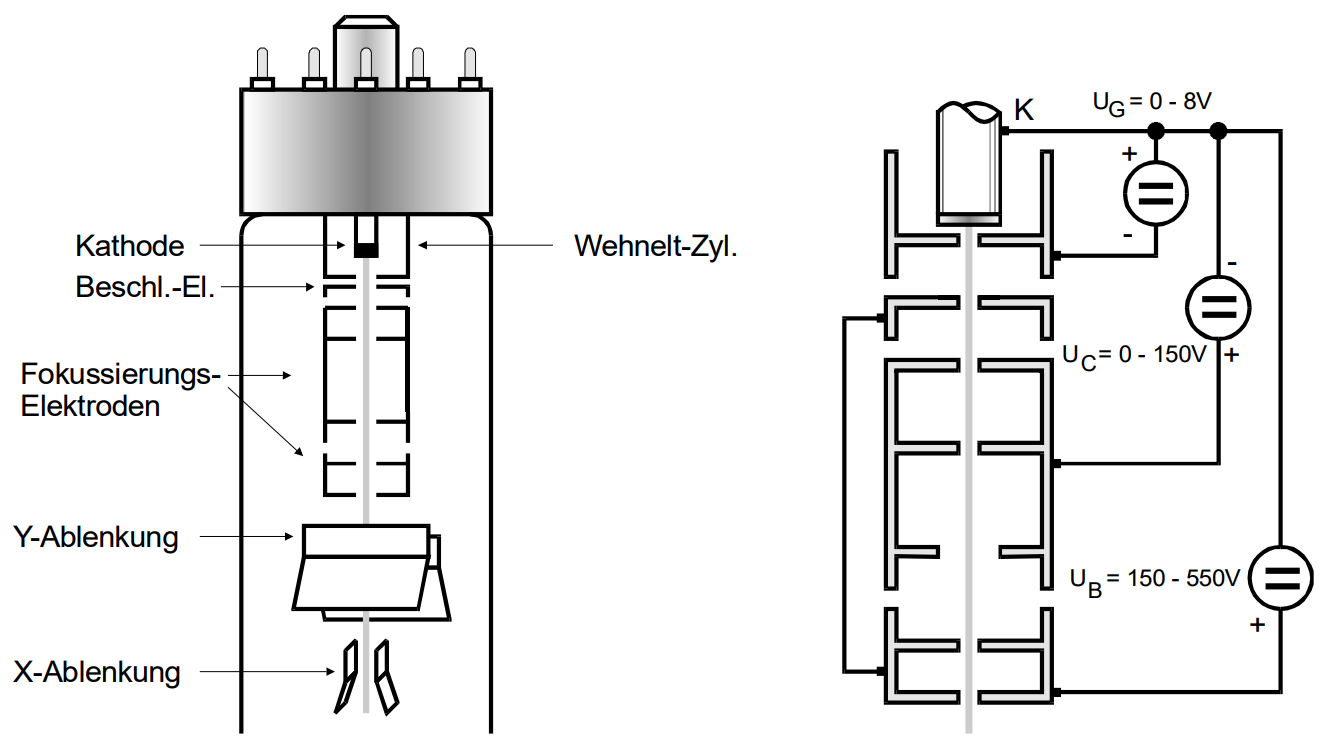
\includegraphics[width=400pt]{data/kathodenstrahlroehre.png}
  \caption{Darstellung einer Kathodenstrahlröhre und Schaltbild einer Elektronenkanone\cite{Versuchsanleitung501}}
  \label{fig:kathode}
\end{figure}

Durch Glühemission entstehen Elektronen an der Oberfläche einer Kathode. Dazu
wird ein Draht in der Kathode bis zur Rotglut erhitzt. Der sogenannte Wehnelt-Zylinder
umgibt die Kathode. Er verfügt über ein zur Kathode negatives elektrisches Potenzial, sodass diese durch eine Bohrung geführt werden. Die Intensität
des Strahls kann durch dieses Potenzial eingestellt werden.
Dann folgt eine Elektrode, die durch ein hohes positives Potenzial $U_\text{B}$
die Elektronen des Strahls beschleunigt. Es ergibt sich eine Geschwindigkeit $v_z$,
die sich durch Anwendung des Energieerhaltungssatzes zu
\begin{equation}
  \frac{m_0 v_z^2}{2} = e_0 U_\text{B}
  \label{eqn:energie}
\end{equation}
ergibt. Dabei bezeichnet $e_0$ die Elementarladung und $m_0$ die Elektronenmasse.
Es werden nichtrelativistische Geschwindigkeiten angenommen.
Die Elektronen durchlaufen weitere Elektroden, deren inhomogene Felder den Strahl
gezielt auf den Leuchtschirm fokussieren. Dies wird Elektronenlinse genannt. Ihre
Brechkraft lässt sich über die Spannung $U_\text{C}$ regeln. In der Oberfläche des Leuchtschirms
werden durch das Auftreffen der Elektronen Aktivatorzentren angeregt, sodass die
Auftrefforte durch Lichtemission sichtbar werden.
Die Ablenkung des Elektronenstrahls erfolgt durch das Ablenksystems. Dieses besteht aus
zwei Paaren von Ablenkplatten, an die eine Spanung angelegt wird. Dadurch entsteht ein elektrisches
Feld, welches den Elektronenstrahl ablenken kann und die Lage des Leuchtflecks auf
dem Schirm verschiebt.

\subsection{Ablenkung eines Elektronstahls im elektrischen Feld}
\label{subsec:Ablenkungtheorie}
Konkret hängt die Ablenkung $D$ geladener Teilchen von der elektrischen Feldstärke $E$
und der Teilchengeschwindigkeit ab.
Eine Skizze der Strahlablenkung in der Kathodenstrahlröhre ist in Abbildung \ref{fig:ablenkungtheorie}
zu sehen.

\begin{figure}[H]
  \centering
  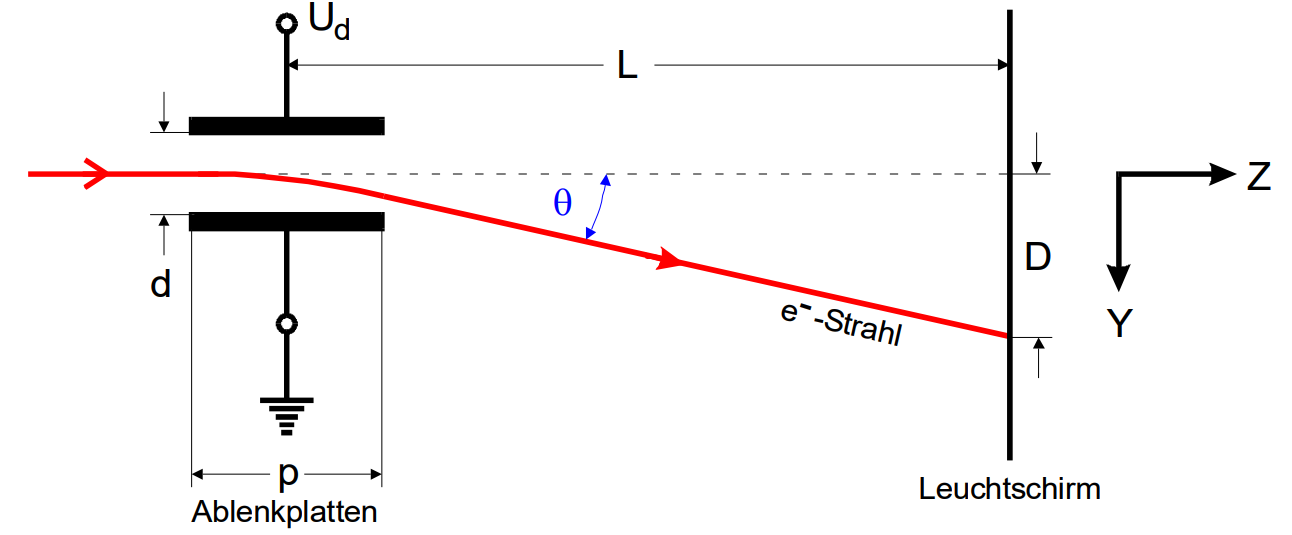
\includegraphics[width=350pt]{data/strahlablenkung.png}
  \caption{Darstellung der Ablenkung des Elektronenstrahls in der Kathodenstrahlröhre.\cite{Versuchsanleitung501}}
  \label{fig:ablenkungtheorie}
\end{figure}

Mit der Näherung $d \ll p$ ist das elektrische Feld zwischen den Ablenkplatten näherungsweise
homogen und es gilt für die elektrische Feldstärke
\begin{equation}
  E = \frac{U_d}{d}\,.
  \label{eqn:EUd}
\end{equation}
Für die Kraft $F$ auf ein geladenes Teilchen im elektrischen Feld gilt dann
\begin{equation}
  F = e_0 E = e_0 \frac{U_d}{d}\,.
  \label{eqn:Fe0E}
\end{equation}
Da sich das Elektron in horizontaler Richtung gleichförmig mit der Geschwindigkeit
$v_z$ bewegt, gilt mit der Plattenlänge $p$ für die Durchlaufzeit durch das Feld
\begin{equation}
  \Delta t = \frac{p}{v_z}\,.
  \label{eqn:deltat}
\end{equation}
Für die Geschwindigkeit in $y-\text{Richtung}$ ergibt sich dann mit den Gleichungen
\eqref{eqn:Fe0E} und \eqref{eqn:deltat}
\begin{equation}
  v_y = \frac{1}{m_0} F \Delta t = \frac{e_0}{m_0}\frac{U_d}{d}\frac{p}{v_z}\,.
  \label{eqn:vy}
\end{equation}
Für den Ablenkwinkel $\Theta$ gilt in Kleinwinkelnäherung $\Theta \approx \frac{v_y}{v_z}$, sodass
mit \eqref{eqn:vy} für die Verschiebung $D$ des Leuchtflecks
\begin{equation}
  D = L \Theta = \frac{e_0}{m_0} L \frac{U_d}{d}\frac{p}{v_z^2}\,.
\end{equation}
gilt. Unter Verwendung von \eqref{eqn:energie} folgt schlussendlich
\begin{equation}
  D = \frac{p}{2d} L \frac{U_d}{U_B}\,.
\end{equation}
Es stellt sich also heraus, dass die Ablenkung $D$ proportional zur Ablenkungspannung
$U_d$ ist.
\subsection{Der Kathodenstrahl-Oszillosgraph}
\label{subsec:oszi}
Ein Kathodenstrahl-Oszillosgraph stellt die Zeitabhängigkeit von Wechselspannungen dar.
Dazu wird an die Ablenkplatten der Kathodenstrahlröhre eine Sägezahnspannung für die
horizontale Ablenkung verwendet. An die vertikal ablenkenden Platten wird die zu untersuchende
Spannung angelegt.
